\renewcommand{\portraitsize}{4cm}
A list of all vehicles present in the X series. Artworks from~\cite{book:MMX_Complete_art}
\begin{itemize}
	\item \hypertarget{vehicle:Death_Rogumer}{\textbf{Death Rogumer:}}
	An Aerial battleship made for the Maverick Hunter's air cavalry. Originally made in order to hold down reploid rebellions, Sigma converted it as a fortress 
	for his army, entrusting the command to the former leader of 7th Airborne unit, Storm Eagle~\cite{wayback:X_resources}.
	\begin{figure}[htp]
		\centering
		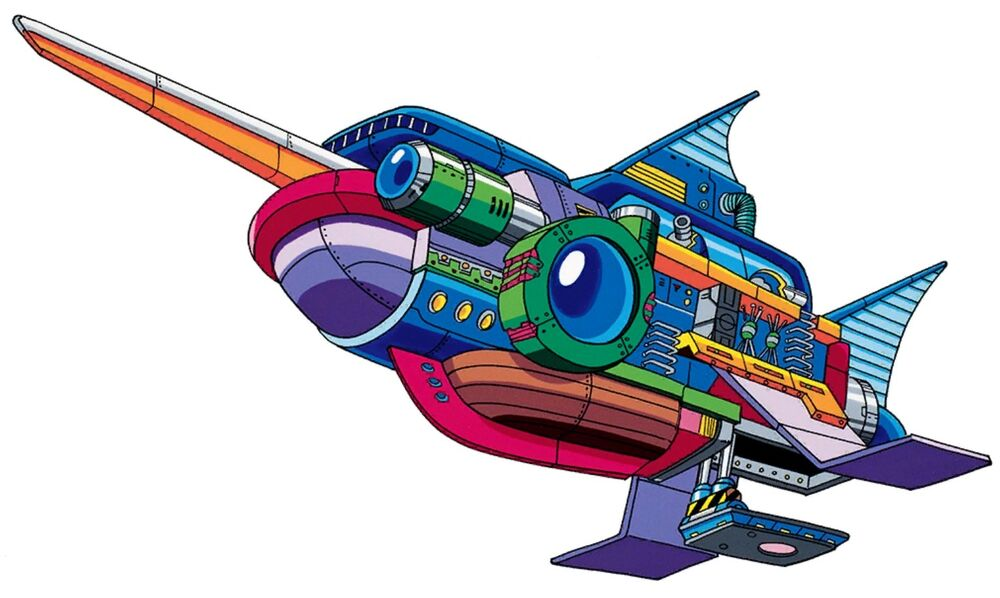
\includegraphics[height=\portraitsize]{figures/X1/Storm_eagle/DeathRogumer.jpg}
		\caption{Death Rogumer}
	\end{figure}
	\item \hypertarget{vehicle:Ride_Armor}{\textbf{Ride Armor:}}
	Ride Armors are mechas similar to tanks with attached hands and feet. Originally these machines were made intended to be used in engineering~\cite{wayback:X_resources}, but were later used also for fighting, as they greatly increase the power of their user due being able to dash, walk over spikes, deliver powerful attacks and receive damage in place of 
	their pilot. Starting from this base version many others will be created, focused more on combat power. Vile himself uses two modified Ride Armors in his confrontation with X, although both of them were destroyed by Zero.
	\begin{figure}[htp]
		\centering
		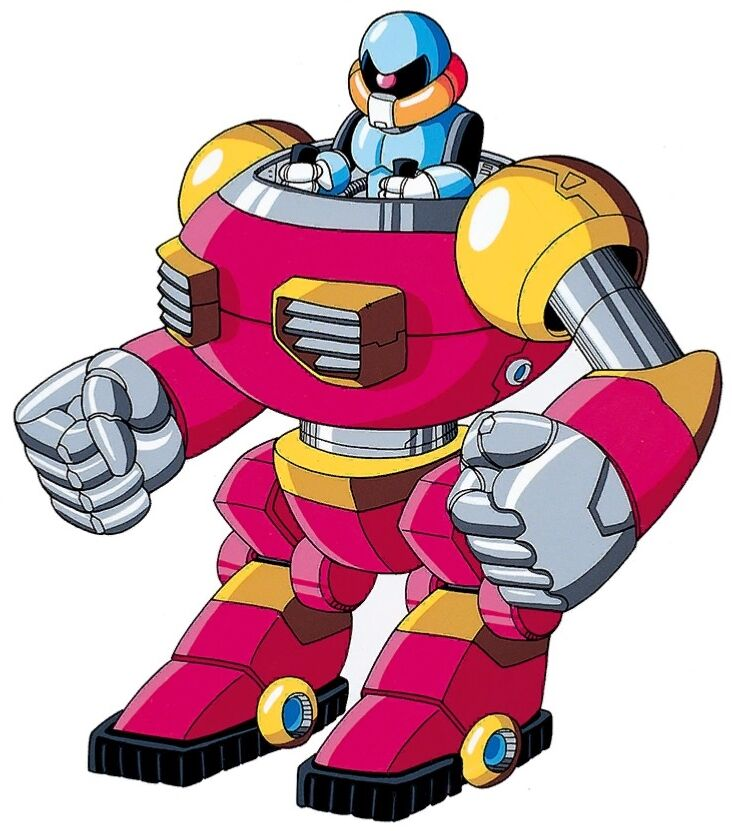
\includegraphics[height=\portraitsize]{figures/X1/Enemies/ArmorSoldier.jpg}
		\caption{Ride Armor 's artwork (with pilot)}
	\end{figure}
	
	\item \hypertarget{vehicle:Ride_Armor_Rabbit}{\textbf{Ride Armor EG-2 custom ``\textit{Rabbit}'':}}
	Upgraded version of the original ride armor drove by Vile and X. It is  equipped with drill hands for mine excavation, and jets attached to its back for improved, although limited, flight ability~\cite{wayback:X2_resources}. 
	\begin{figure}[htp]
		\centering
		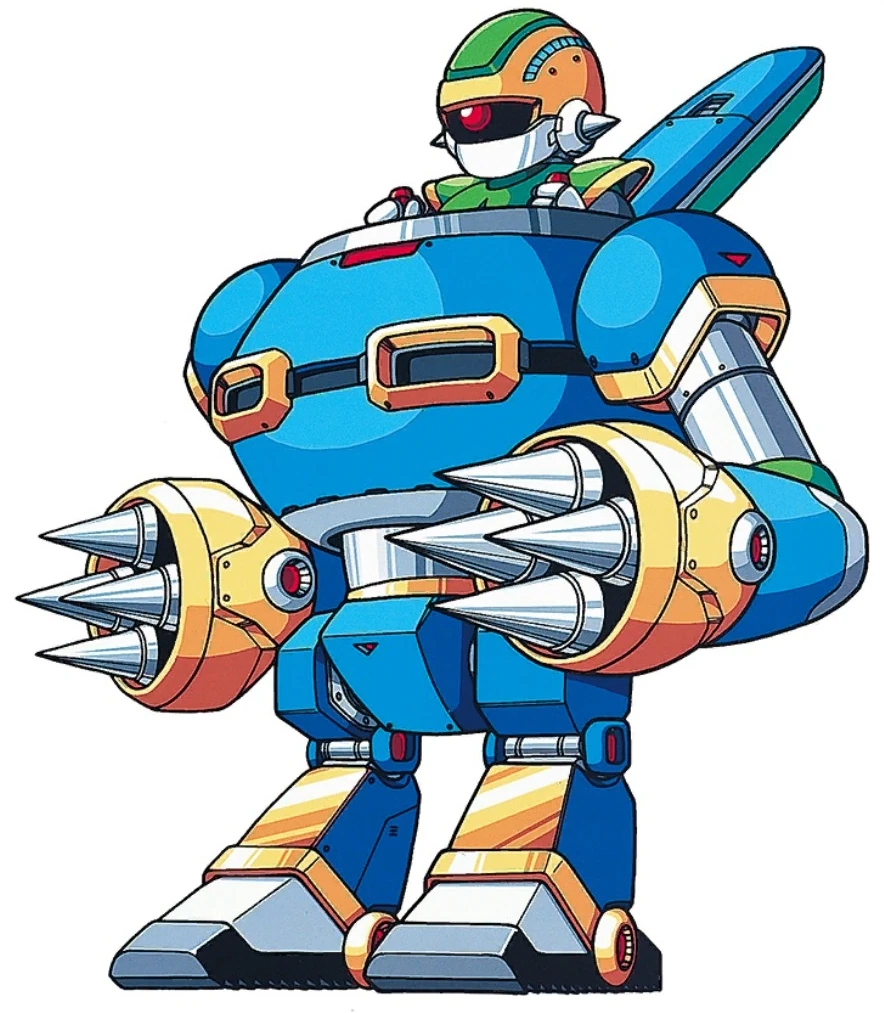
\includegraphics[height=\portraitsize]{figures/X2/Enemies/Ride_armor_RABBIT.png}
		\caption{Ride Armor RABBIT}
	\end{figure}
	
	\item \hypertarget{vehicle:Ride_Armor_Chimera}{\textbf{Ride Armor type DRA-00 ``\textit{Chimera}'':}} Default form of the general purpose Ride Armor DRA-00. It provides average mobility, but it can be customized using different modules. In the game's manual it was stated that Dr.~Light had created the custom modules~\cite{X3:Manual}, but it was later changed to be a creation of the Maverick Hunters~\cite{book:Compendium}.
%	\begin{figure}[htp]
%		\centering
%		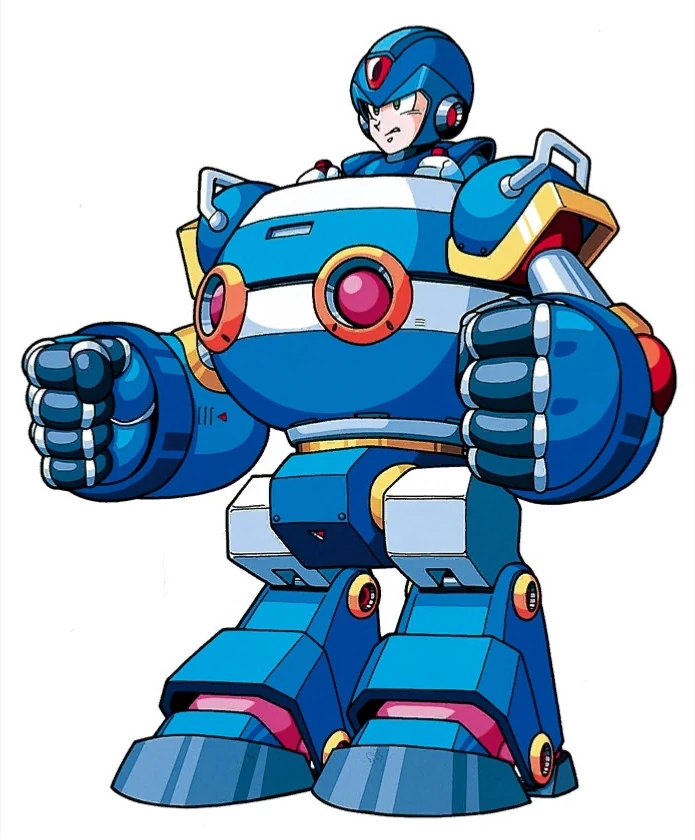
\includegraphics[height=\portraitsize]{figures/X3/weapons/Chimera.png}
%		\caption{Ride Armor Chimera}
%	\end{figure}
	
	\item \hypertarget{vehicle:Ride_Armor_Frog}{\textbf{Ride Armor ``\textit{Frog}'':}} The first aquatic ride armor, Named because of its hopping movement, it is difficult to 
	handle on the ground, but very easy in the water. It is armed with homing torpedo~\cite{wayback:X3_resources}.
%	\begin{figure}[htp]
%		\centering
%		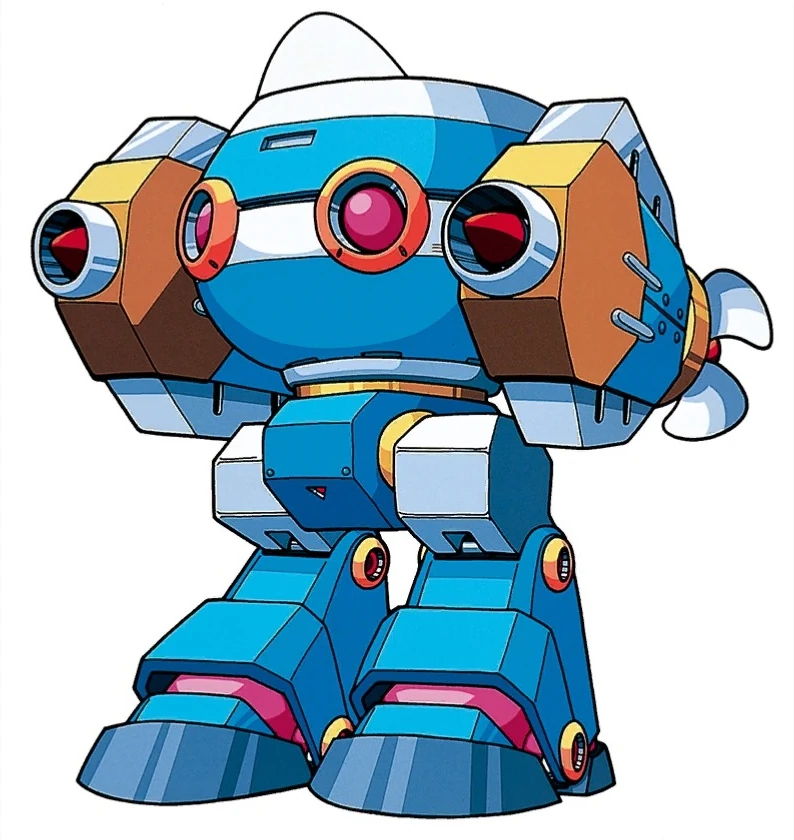
\includegraphics[height=\portraitsize]{figures/X3/weapons/Frog.png}
%		\caption{Ride Armor - Frog Module}
%	\end{figure}
	
	\item \hypertarget{vehicle:Ride_Armor_Kangaroo}{\textbf{Ride Armor ``\textit{Kangaroo}'':}} Ride Armor equipped with rotating drills on each arm, to improve its combat efficiency. When charged up, it can use the Spinning Claw attack, firing its claws with a chain attached to it~\cite{wayback:X3_resources,book:MH_field_guide}. Vile mk.II uses a black version of this armor in his first confrontation.
%	\begin{figure}[htp]
%		\centering
%		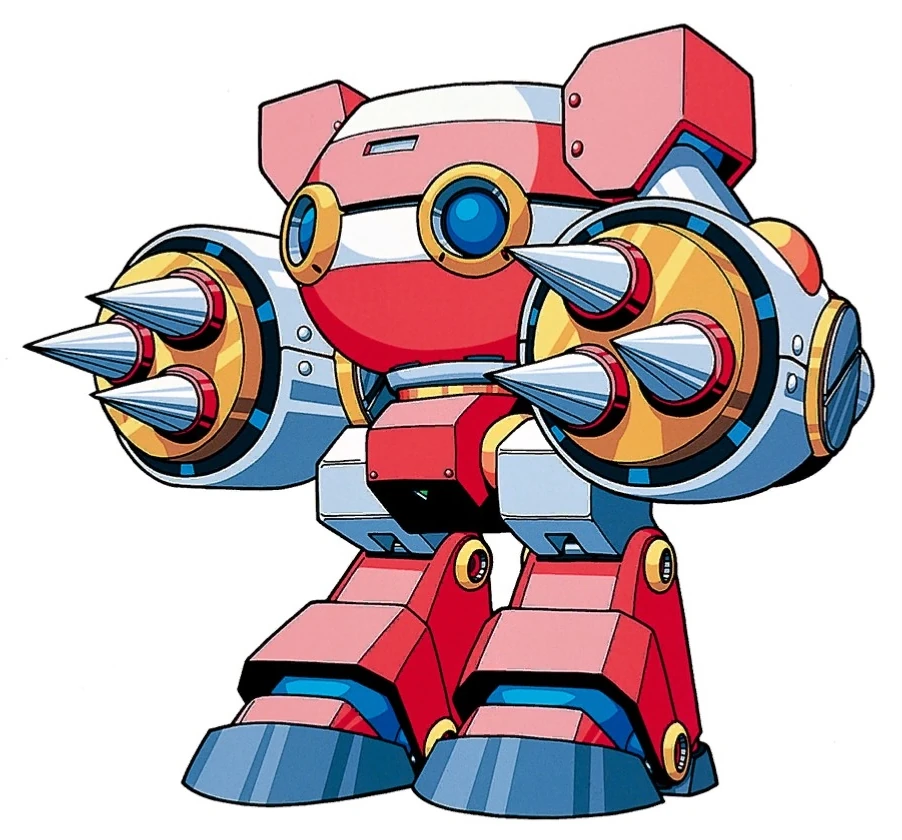
\includegraphics[height=\portraitsize]{figures/X3/weapons/Kangaroo.png}
%		\caption{Ride Armor - Kangaroo Module}
%	\end{figure}
	
	\item \hypertarget{vehicle:Ride_Armor_Hawk}{\textbf{Ride Armor ``\textit{Hawk}'':}} Ride armor with superior air mobility. Its hovering function exceeds even that of the previous RABBIT model, substituting the jets with a large hover-fan~\cite{book:MH_field_guide}. It is armed with the homing missile~\cite{wayback:X3_resources}.
%	\begin{figure}[htp]
%		\centering
%		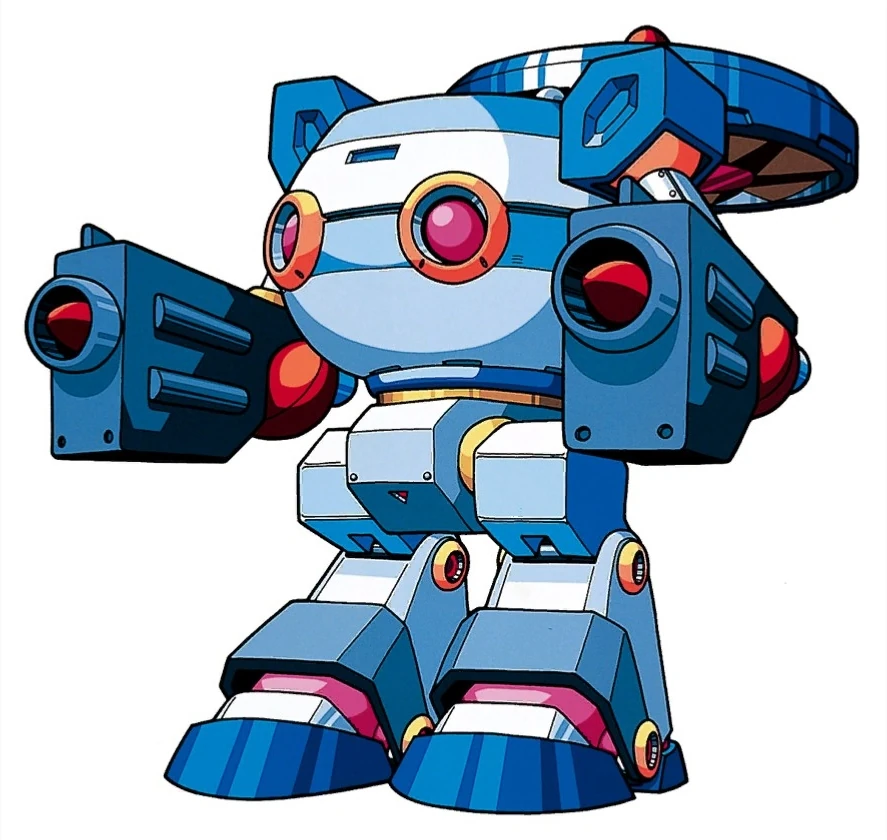
\includegraphics[height=\portraitsize]{figures/X3/weapons/Hawk.png}
%		\caption{Ride Armor - Hawk Module}
%	\end{figure}
	
	\begin{figure}[htp]
		\centering
		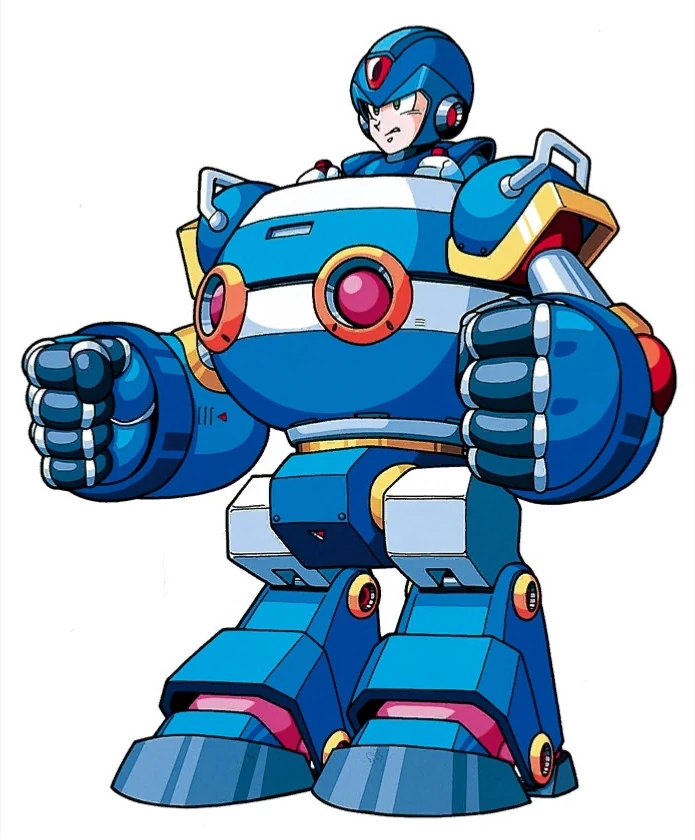
\includegraphics[height=\portraitsize]{figures/X3/weapons/Chimera.png}
		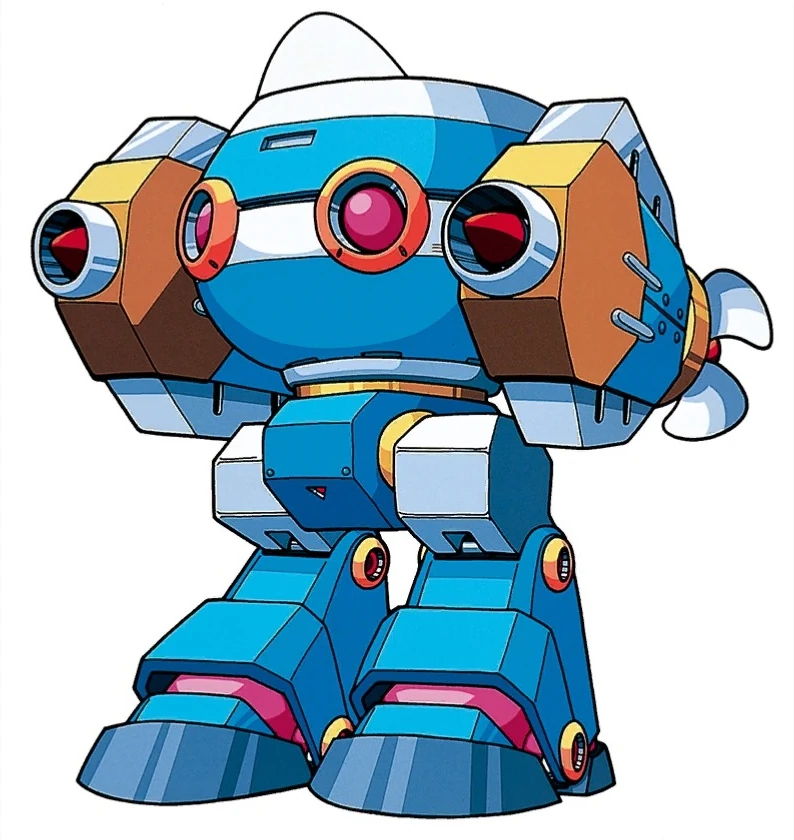
\includegraphics[height=\portraitsize]{figures/X3/weapons/Frog.png}\\
		\vspace{2pt}
		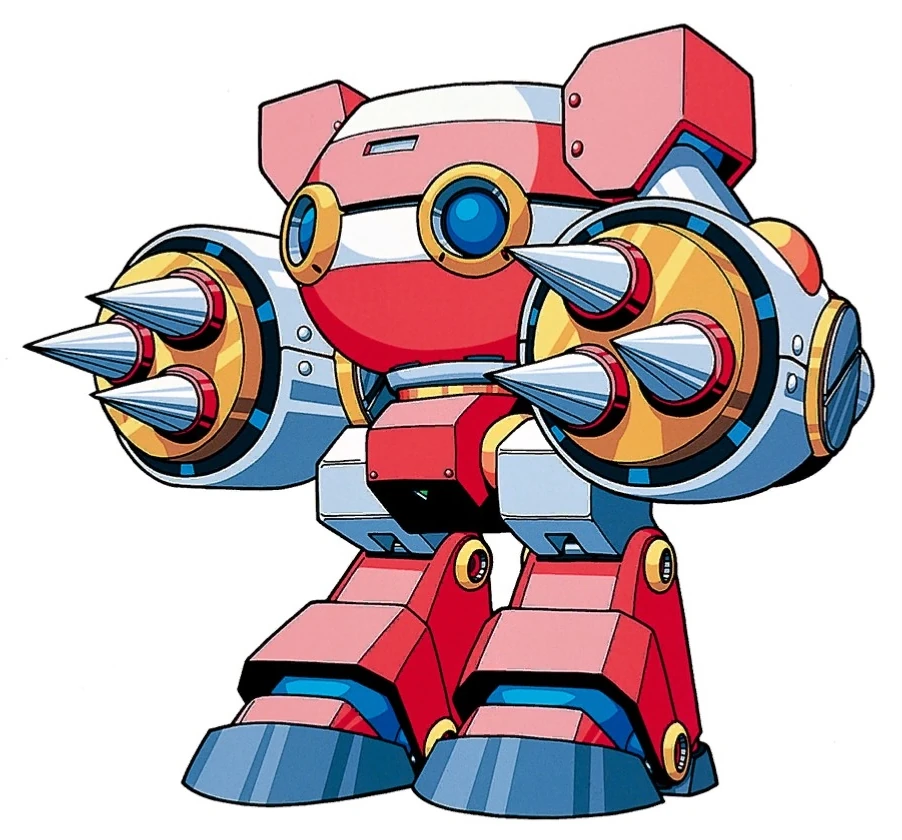
\includegraphics[height=\portraitsize]{figures/X3/weapons/Kangaroo.png}
		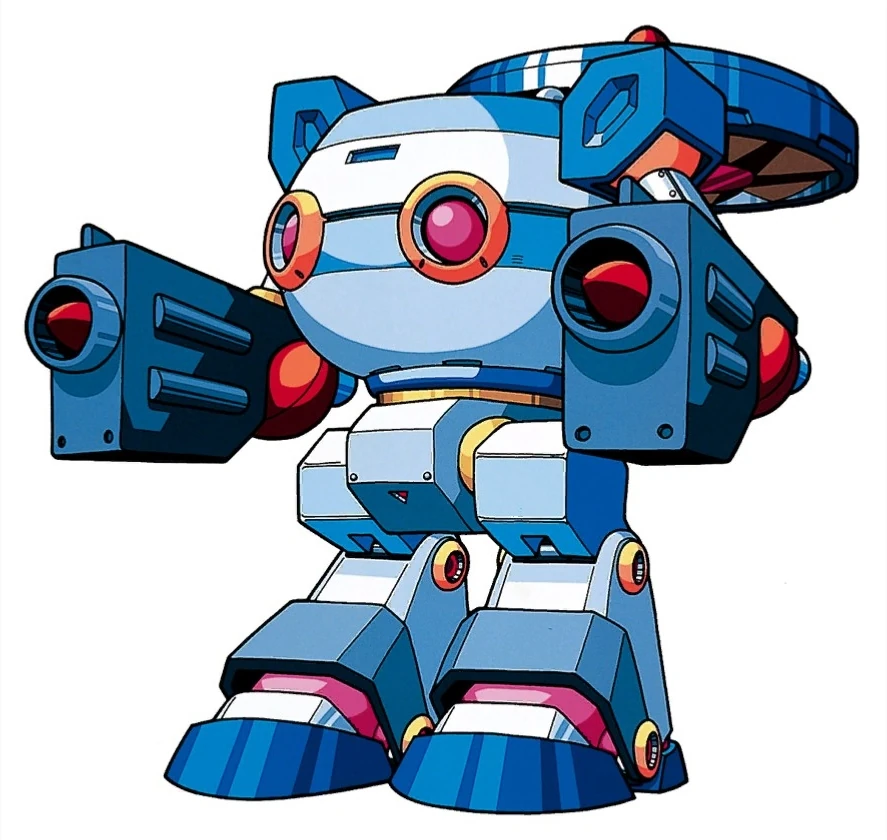
\includegraphics[height=\portraitsize]{figures/X3/weapons/Hawk.png}
		\caption{Ride Armor modules : Chimera, Frog, Kangaroo, Hawk}
	\end{figure}
	
	\item \hypertarget{vehicle:Ride_Armor_Goliath}{\textbf{Ride Armor ``\textit{Goliath/Brown Bear}'':}} The custom ride armor used by Vile Mk.II at Doppler's lab. Different from 
	other Ride Armors, it was designed specifically for combat~\cite{wayback:X3_resources}. According to Vile, the Goliath is the world's most advanced Ride Armor.~\cite{book:MH_field_guide}
	\begin{figure}[htp]
		\centering
		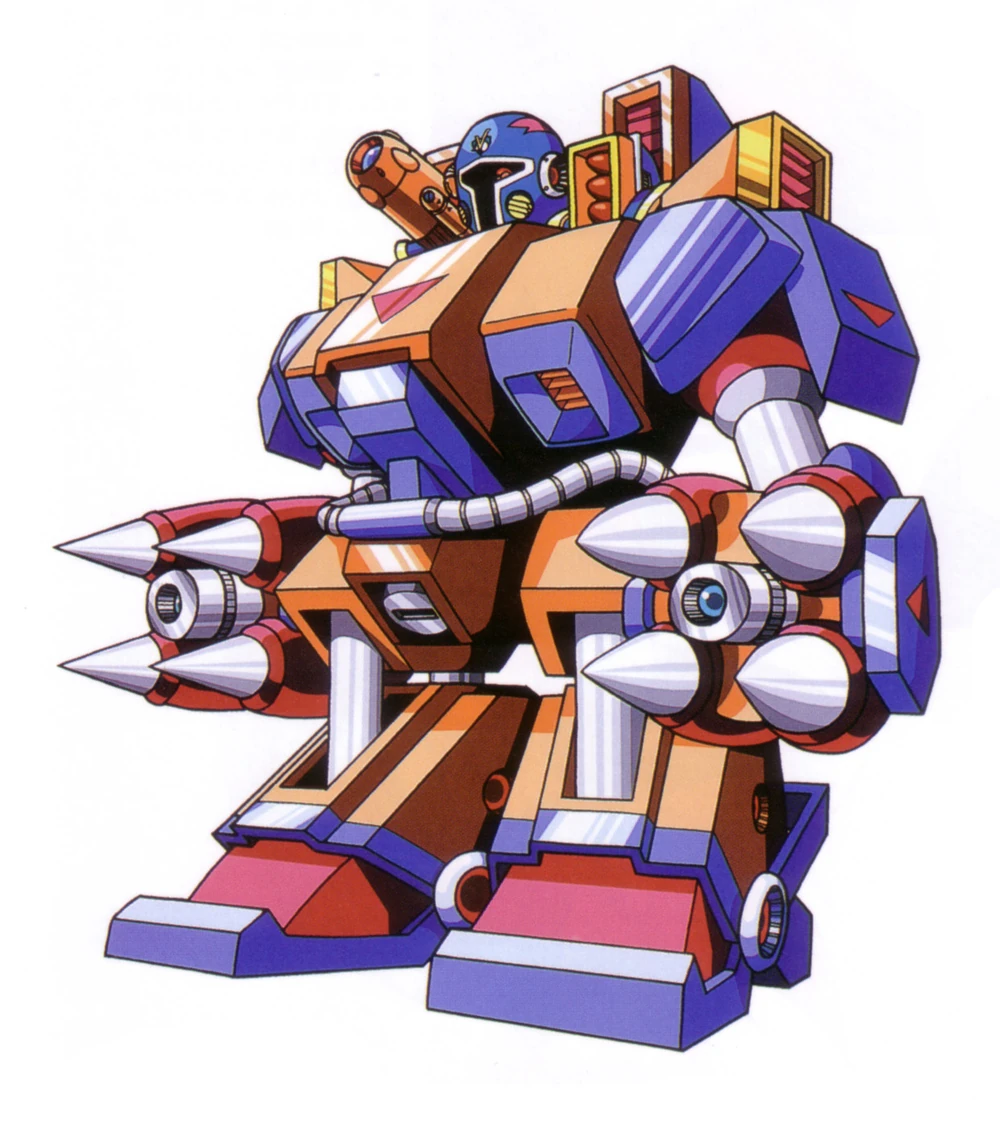
\includegraphics[height=\portraitsize]{figures/X3/Doppler_stages/vile2_armor.png}
		\caption{Ride Armor Golitath/Brown Bear and Vile}
	\end{figure}
	
	
	\item \hypertarget{vehicle:Ride_Chaser_Cheval}{\textbf{Ride Chaser ADU-T400 turbo "\textit{Cheval}": }}
	Reploid private air bike. Designed for running at extreme speeds, 
	it is a super advanced vehicle with a useful Turbo function. Weak to impact, due to a fault it instantly self-destruct upon striking on something~\cite{wayback:X2_resources}.
	\begin{figure}[htp]
		\centering
		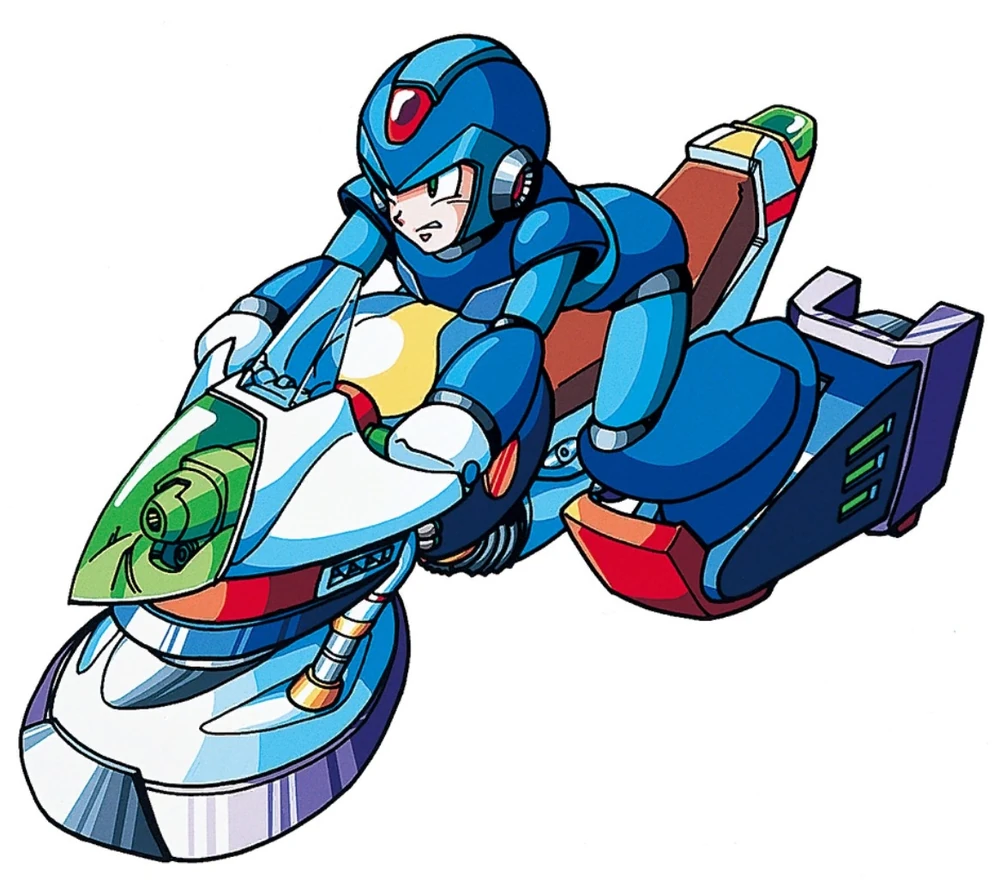
\includegraphics[height=\portraitsize]{figures/X2/weapons/RCCheval.png}
		\caption{Ride Chaser ``Cheval''}
	\end{figure}
	
	
	
	
\end{itemize}


